% \documentclass[tikz,convert={outfile=\jobname.svg}]{standalone}
\documentclass[tikz,convert=pdf2svg]{standalone}
%\usetikzlibrary{...}% tikz package already loaded by 'tikz' option
\usetikzlibrary{arrows, arrows.meta}
% \tikzset{
%   >=stealth',
% }
\usepackage{amsmath,amssymb}
\usepackage{tikz}
\usepackage{xcolor}

\begin{document}
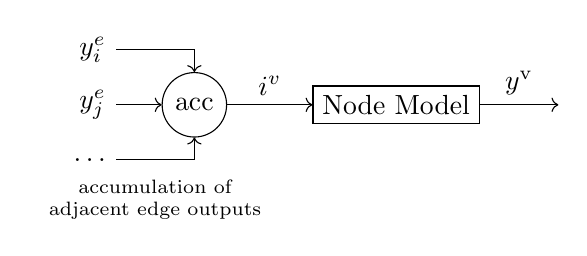
\begin{tikzpicture}
  \node[draw](n){
    Node Model
  };
  \draw[->](n.east)--++(1.0,0) node[above, pos=.5]{$y^{\mathrm v}$};
  
  % Draw the accumulator circle
  \node[draw, circle] (acc) at ([xshift=-1.5cm]n.west) {$\mathrm{acc}$};
  
  % Connect acc to the node
  \draw[->] (acc) -- (n.west) node[pos=.5, above]{$i^{v}$};
  
  % Add three arrows to acc with rectangular corners
  \draw[<-] (acc) |- ++(-1.0,0.7) node[left](in){$y^e_i$};
  \draw[<-] (acc) -- ++(-1.0,0) node[left]{$y^e_j$};
  \draw[<-] (acc) |- ++(-1.0,-0.7) node[left]{$\ldots$};
  
  % Add a label for the accumulation function
  \node[text width=3cm, align=center, font=\scriptsize] at ([xshift=-.5cm, yshift=-1.2cm]acc) {accumulation of adjacent edge outputs};

\end{tikzpicture}
\end{document}
